% 18W MOSFET amplifier, with npn transistor.
% Author: Ramón Jaramillo.
\documentclass[margin=10pt]{standalone}
%%%<
\usepackage{verbatim}
%%%>
\begin{comment}
:Title: 18W MOSFET amplifier with npn transistor
:Tags: Circuits;circuitikz;Electrical engineering
:Author: Ramón Jaramillo
:Slug: mosfet

This example make use of the circuitikz and siunitx packages for drawing
a 18W MOSFET  Amplifier for one-channel. You need to have those packages
installed for compiling.

Source: http://www.circuitstoday.com/mosfet-amplifier-circuits
\end{comment}
\usepackage[siunitx]{circuitikz}
\begin{document}
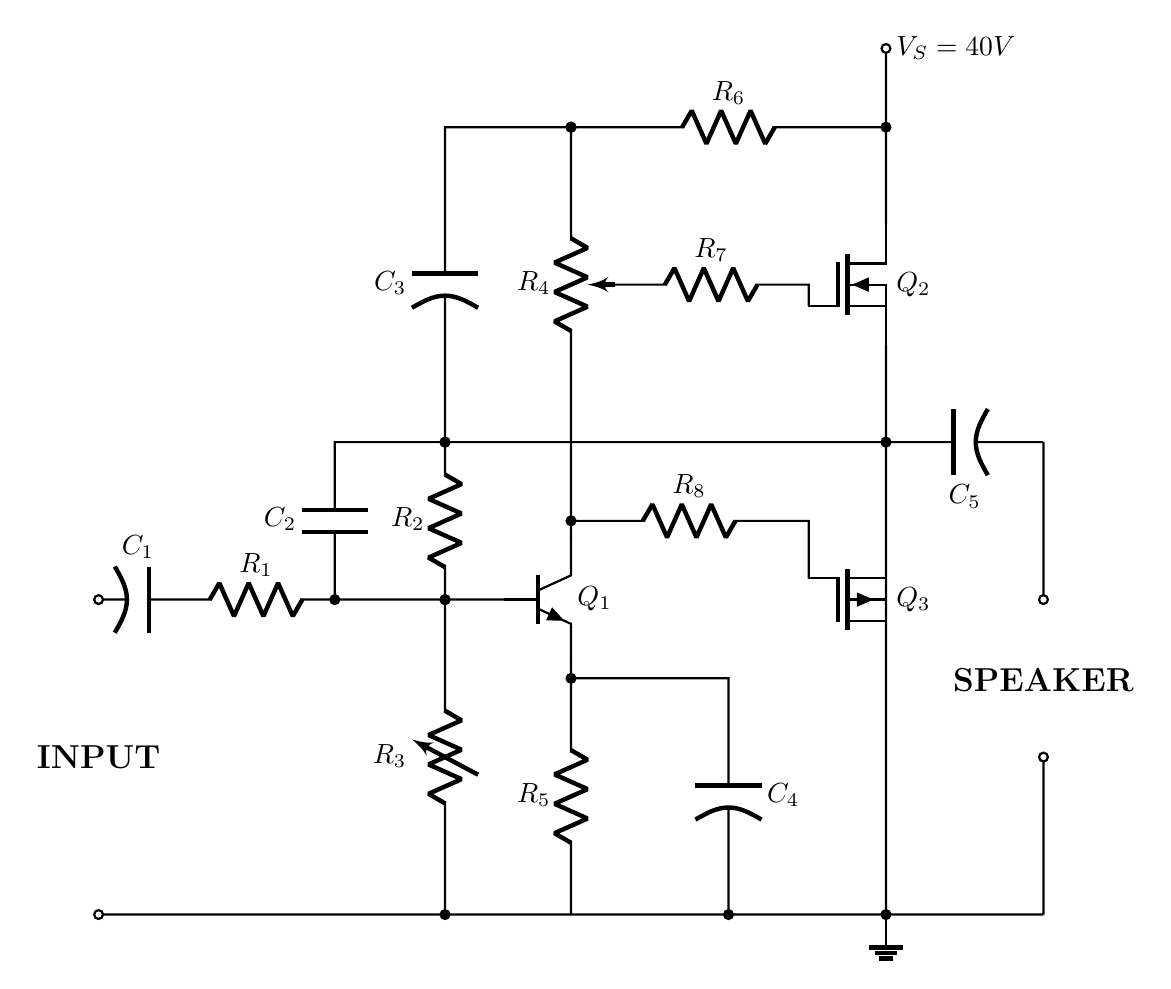
\begin{tikzpicture}[scale=2]
  \draw[color=black, thick]
    (0,0) to [short,o-] (6,0){} % Baseline for connection to ground
    % Input and ground
    (0,1) node[]{\large{\textbf{INPUT}}}
    % Connection of passive components
    (5,0) node[ground]{} node[circ](4.5,0){}
    (0,2) to [pC, l=$C_1$, o-] (0.5,2)
    to [R,l=$R_1$,](1.5,2)
    to node[short]{}(2.6,2)
    (1.5,2) to [C, l=$C_2$, *-] (1.5,3) -| (5,3)
    (2.2,2) to [R, l=$R_2$, *-*] (2.2,3)
    (2.2,3) to [pC, l=$C_3$, *-] (2.2,5) -| (3,5)
    % Transistor Bipolar Q1
    (3,0) to [R,l=$R_5$,-*] (3,1.5)
    to [Tnpn,n=npn1] (3,2.5)
    (npn1.E) node[right=3mm, above=5mm]{$Q_1$} % Labelling the NPN transistor
    (4,0) to [pC, l_=$C_4$, *-] (4, 1.5)--(3,1.5)
    (2.2,0) to [vR, l=$R_3$, *-*] (2.2,2)
    (3,2.5) to node[short]{}(3,3)
    (3,5) to [pR, n=pot1, l_=$R_4$, *-] (3,3)
    (3,5) to [R, l=$R_6$, *-] (5,5)
    to [short,*-o](5,5.5) node[right]{$V_S=40 V$}
    % Mosfet Transistors
    (5,3) to [Tnigfetd,n=mos1] (5,5)
    (mos1.B) node[anchor=west]{$Q_2$} % Labelling MOSFET Q2 Transistor
    (pot1.wiper)  to [R, l=$R_7$] (4.5,4) -| (mos1.G)
    (5,1.5) to [Tpigfetd,n=mos2] (5,2.5)
    (5,0) to (mos2.S)
    (3,2.5) to [R, l=$R_8$, *-] (4.5,2.5)
    -| (mos2.G)
    (mos2.B) node[anchor=west]{$Q_3$} % Labelling MOSFET Q3 Transistor
    % Output
    (6,3) to [pC, l=$C_5$,-*](5,3)
    (6,3) to [short,-o] (6,2){}
    (mos1.S)--(mos2.D)
    (6,0) to [short,-o] (6,1){} node[above=7mm]{\large{\textbf{SPEAKER}}}
    ;
\end{tikzpicture}
\end{document}
